This section discusses the analysis performed on Airline data which was preseted at Data expo 2008. Analysis of data is performed in R and ggplot library is used for presenting the graphical charts.

\section{Evaluting Traffic Patterns of top Metropolitan Cities}\begin{figure}[htp]
\centering
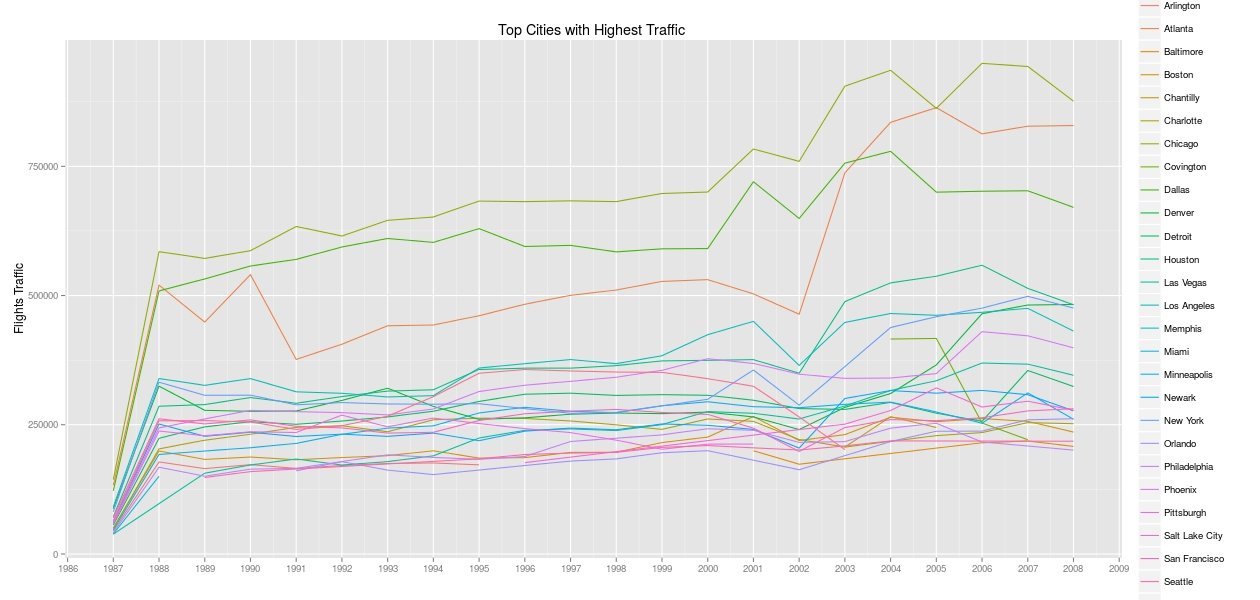
\includegraphics[scale=0.3]{/home/perfectus/Documents/Rworkspace/presentation/HighestTraffic20yrsCities.jpeg}
\caption{}
\label{fig1}
\end{figure}

We investigated and visualize data for domestic flights that originated or terminated at all cities. We can look at the change in flight traffic patterns because of the increasing populations.
As of April 26, 2015, the United States has a total resident population of 320,760,000, making it the third most populous country in the world.[1] It is very urbanized, with 81\% residing in cities and suburbs as of 2014 (the worldwide urban rate is 54\%).California and Texas are the most populous states,as the mean center of U.S. population has consistently shifted westward and southward.New York City is the most populous city in the United States.

Figure \ref{fig1} displays this three-way comparison of traffic patterns. We have noticed that flight traffic increases with time line but there is a setback in traffic in the year before 2002. Reason for this anomally can be co-realted with 9/11/2001 terrorist attack on WTC. This inturn would have lead to increase in security, more flight regulations and thus heavy decrease in traffic.

\section{Chicago Traffic Pattern}
Chicago, on Lake Michigan in Illinois, is among the largest cities in the U.S. Famed for its bold architecture. The city is also renowned for its museums, including the Art Institute and its expansive collections, including noted Impressionist works.
\subsection{Total Traffic }
\begin{figure}[htp]
\centering
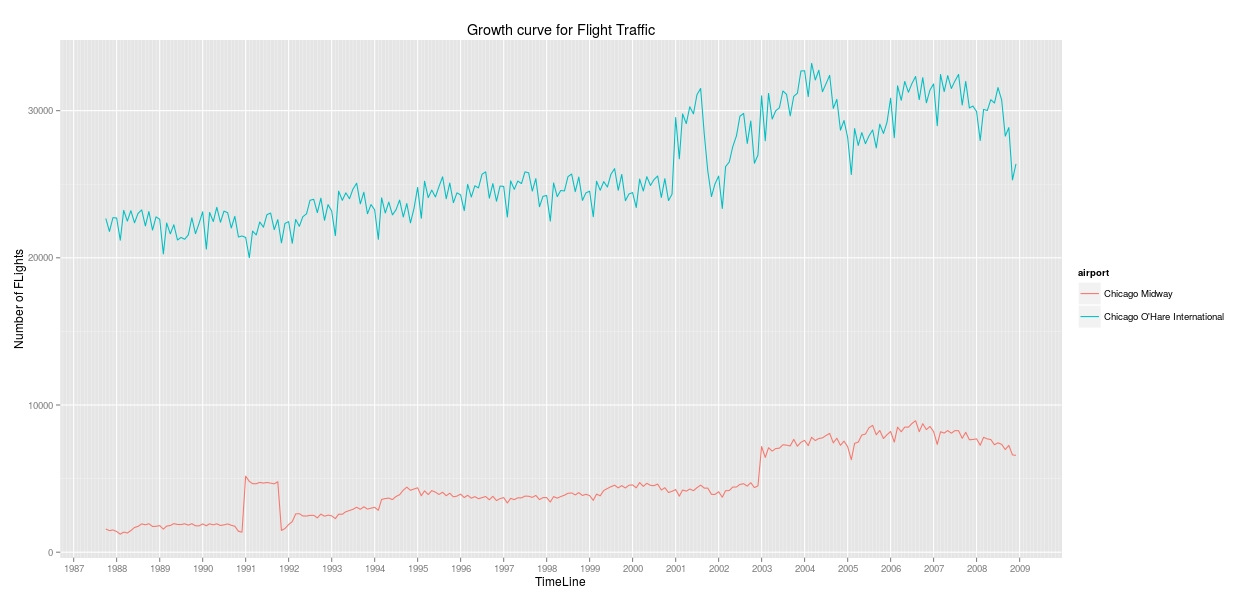
\includegraphics[scale=0.4]{/home/perfectus/Documents/Rworkspace/presentation/chicago-month/ChicagoFlightTraffic.jpeg}
\caption{}
\label{chicago:fig1}
\end{figure}

Figure \ref{chicago:fig1} points the diffrence between two airports of Chicago i.e. Chicago O'Hare and Chicago Midway. Chicago Midway is least used by people of Chicago though O' Hare is one of the busiest airport. We can clearly observer the Chicago Midway traffic growth started from year 2003 when an investment was made to improve the operations on Chicago Midway. Anomally due to 9/11 is less visible in Midway than in O'Hare. 

We can also observe a sharp dip in flight traffic in the month of December and January, this may be because of the Christmas Holidays and New Year eve where most of the pilots would be on leave or because of highly cold weather. 
\subsection{Canceled Flights}
\begin{figure}[htp]
\centering
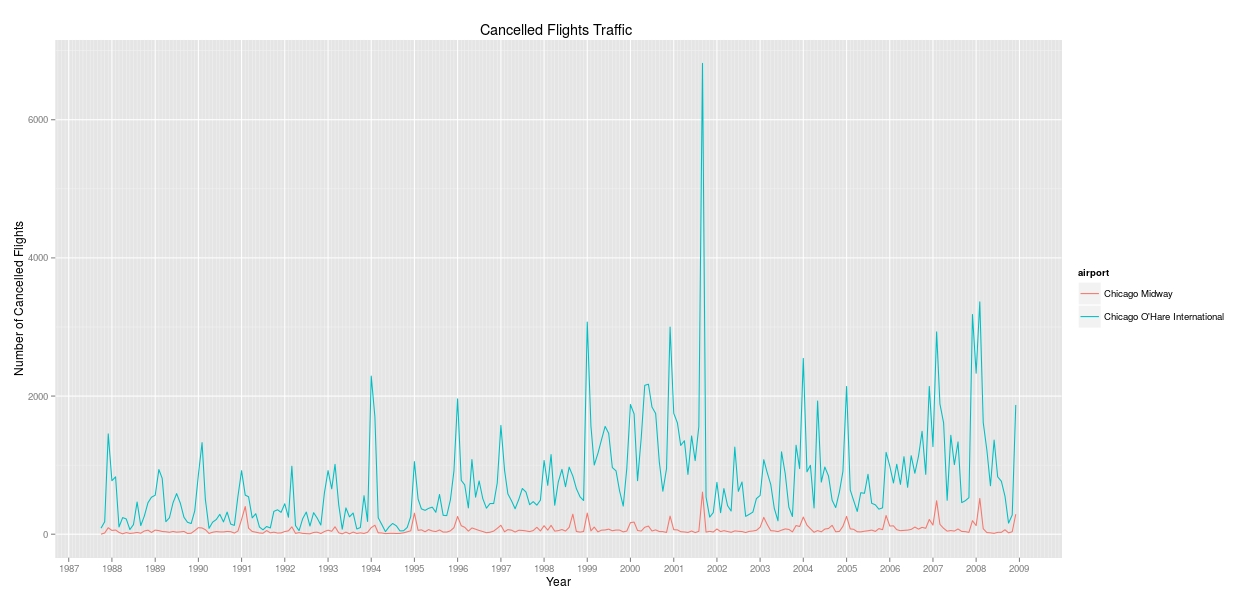
\includegraphics[scale=0.4]{/home/perfectus/Documents/Rworkspace/presentation/chicago-month/ChicagoCancelledFlights.jpeg}
\caption{}
\label{chicago:fig2}
\end{figure}
Figure \ref{chicago:fig2} we can observe the cancellation rate is at peak in the month of December and January. While Figure \ref{chicago:fig1} showed a drop in the same time line.

\subsection{Delay Rate}
\begin{figure}[htp]
\centering
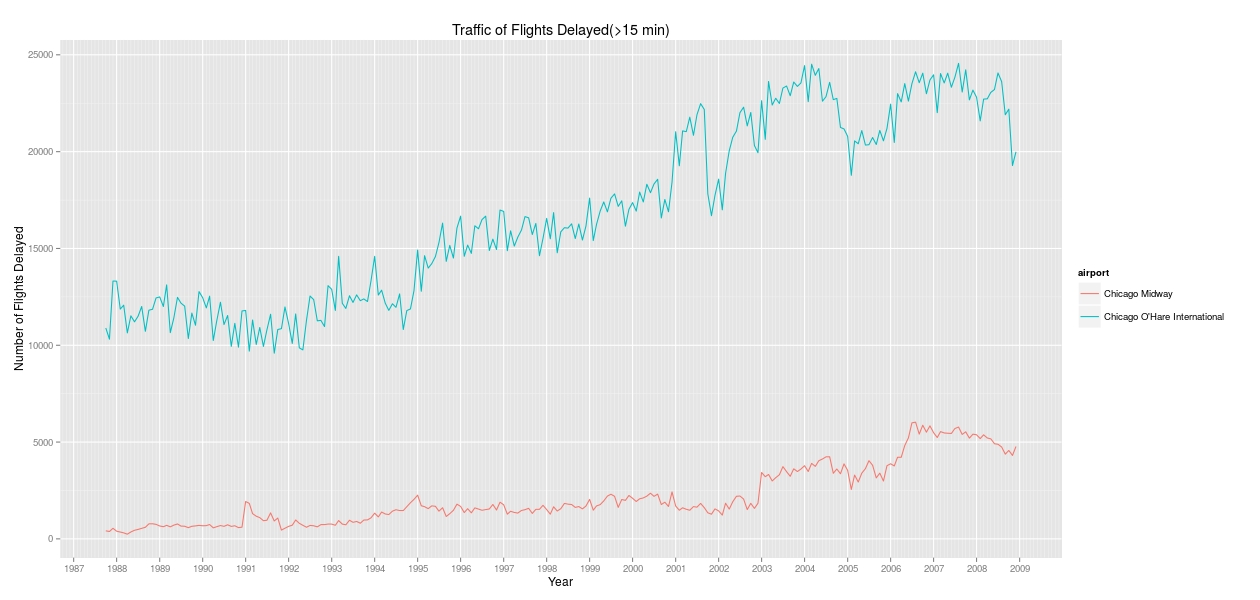
\includegraphics[scale=0.4]{Figures/fig-7.jpeg}
\caption{}
\label{chicago:fig3}
\end{figure}
The graph shown in Figure \ref{chicago:fig3} delay rate pattern for the city Chicago and the diffrence between Midway and O' Hare.

\section{New York Traffic Pattern}
Home to the Empire State Building, Times Square, Statue of Liberty and other iconic sites, New York City is a fast-paced, globally influential center of art, culture, fashion and finance. The analysis is made bewteen LaGaurdia(LGA) and John F Kennedy(JFK).  LGA is a much easier airport to navigate. Unless you're set on taking public transportation to/from the airport its the way to go. LGA is smaller, and thus can be a lot quicker to exit through. It's also much closer to the city than JFK, but this is only useful if you'll be taking a cab. Public transportation from LGA is as good as non-existent.

\subsection{Total Traffic}
In earlier years traffic of LaGuardia was higher than JFK but after advent 2007 JFK has shown higher traffic growth rate. We can also observe lower slope in 2002 because of 9/11. Figure \ref{nyc:fig1} shows steep slope in the start of January 2001 was beacuse of 100th Yankees soccer league.
\begin{figure}[htp]
\centering
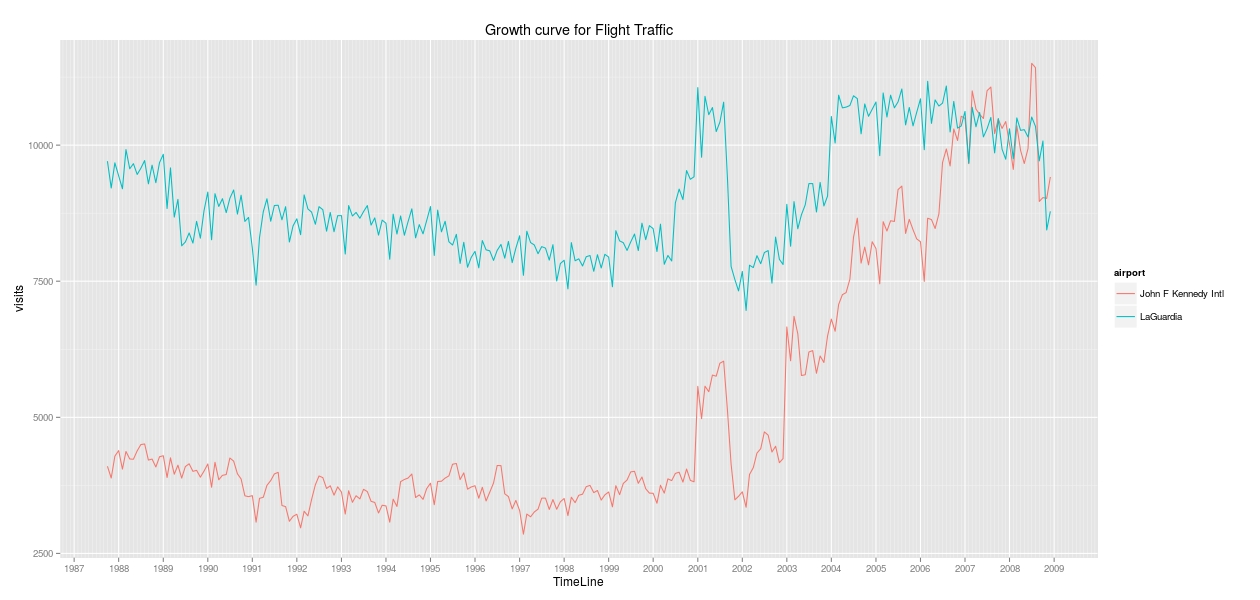
\includegraphics[scale=0.4]{/home/perfectus/Documents/Rworkspace/presentation/nyc-month/NewYork-TrafficAirport-origin.jpeg}
\caption{}
\label{nyc:fig1}
\end{figure}

\subsection{Cancelled Flights}
Figure \ref{nyc:fig2} is shows the cacelled flight status. Similar conclusion can be drawn from this graph as of Figure \ref{chicago:fig2}. High peaks in month of January and 9/11 can be easily observed. 

\begin{figure}[htp]
\centering
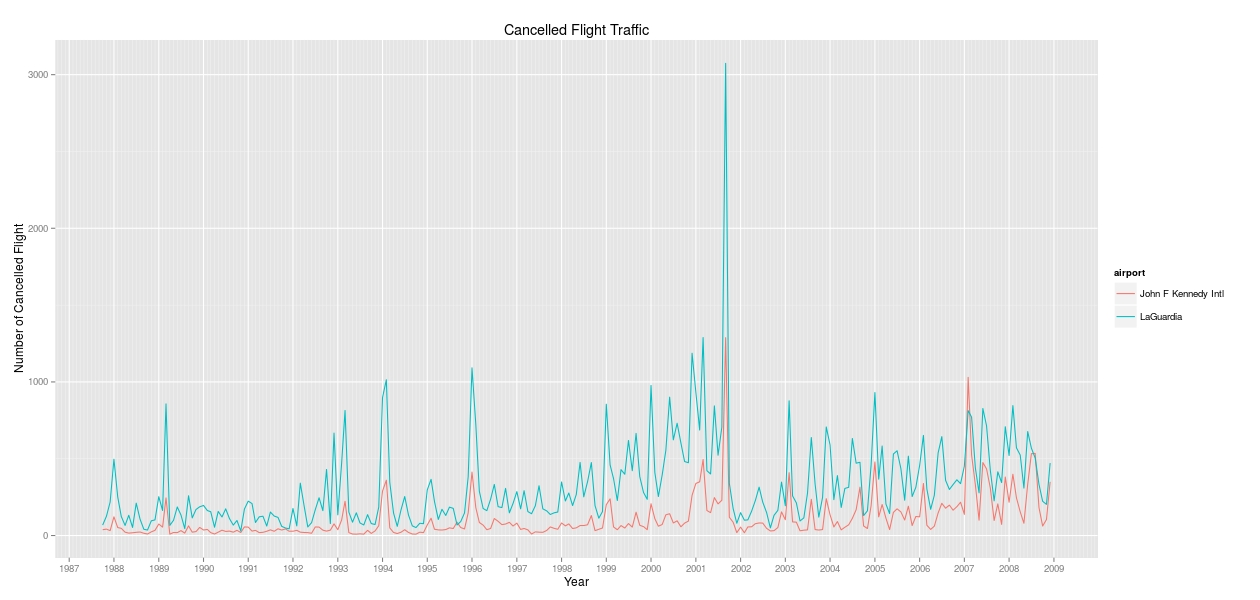
\includegraphics[scale=0.4]{/home/perfectus/Documents/Rworkspace/presentation/nyc-month/Newyork-Cancelelled-months-origin.jpeg}
\caption{}
\label{nyc:fig2}
\end{figure}
\subsection{Delayed Flights}
Figure \ref{nyc:fig3} is imilar to the oberservations made at Chicago. Again similar conclusion can be drawn signifying a general trend in American populations.
\begin{figure}[htp]
\centering
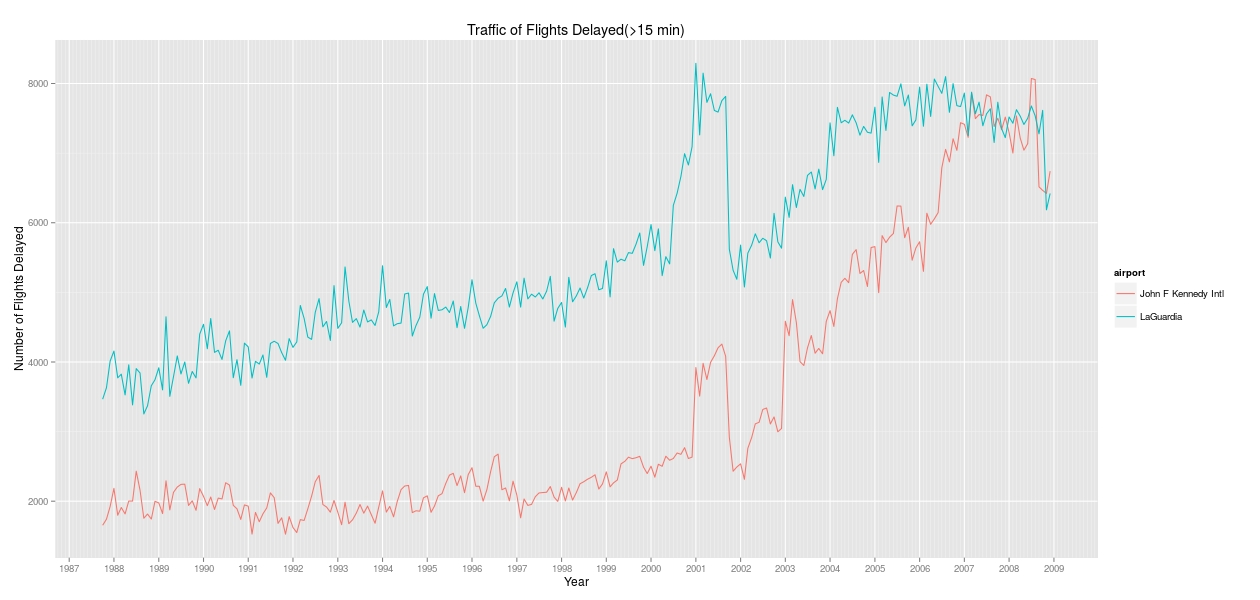
\includegraphics[scale=0.4]{/home/perfectus/Documents/Rworkspace/presentation/nyc-month/NewYork-FlightDelayedOrigin.jpeg}
\caption{}
\label{nyc:fig3}
\end{figure}

